\documentclass[12pt, oneside]{article}

\usepackage[letterpaper, scale=0.89, centering]{geometry}
\usepackage{fancyhdr}
\setlength{\parindent}{0em}
\setlength{\parskip}{1em}

\usepackage{tikz}
\usetikzlibrary{automata,positioning,arrows}

\pagestyle{fancy}
\fancyhf{}
\renewcommand{\headrulewidth}{0pt}
\rfoot{\href{https://creativecommons.org/licenses/by-nc-sa/2.0/}{CC BY-NC-SA 2.0} Version \today~(\thepage)}

\usepackage{amssymb,amsmath,pifont,amsfonts,comment,enumerate,enumitem}
\usepackage{currfile,xstring,hyperref,tabularx,graphicx,wasysym}
\usepackage[labelformat=empty]{caption}
\usepackage{xcolor}
\usepackage{multicol,multirow,array,listings,tabularx,lastpage,textcomp,booktabs}

\lstnewenvironment{algorithm}[1][] {   
    \lstset{ mathescape=true,
        frame=tB,
        numbers=left, 
        numberstyle=\tiny,
        basicstyle=\rmfamily\scriptsize, 
        keywordstyle=\color{black}\bfseries,
        keywords={,procedure, div, for, to, input, output, return, datatype, function, in, if, else, foreach, while, begin, end, }
        numbers=left,
        xleftmargin=.04\textwidth,
        #1
    }
}
{}

\newcommand\abs[1]{\lvert~#1~\rvert}
\newcommand{\st}{\mid}

\newcommand{\cmark}{\ding{51}}
\newcommand{\xmark}{\ding{55}}
 
\begin{document}
\begin{flushright}
    \StrBefore{\currfilename}{.}
\end{flushright} 
\subsection*{Week 2 at a glance}

\subsubsection*{Textbook reading: Sections 1.1, 1.2}

\vspace{-15pt}

Before Monday, read pages 41-43 (Figures 1.18, 1.19, 1.20) for examples of automata and languages.

Before Wednesday, read pages 48-50 (Figures 1.27, 1.29) which introduces nondeterminism.

Before Friday, read pages 60-61 Theorem 1.47 and Theorem 1.48 that we'll refer to as ``closure proofs".

For Week 3 Monday: Theorem 1.39 ``Proof Idea'', Example 1.41, Example 1.56, Example 1.58.


\subsubsection*{We will be learning and practicing to:}
\begin{itemize}
\item Clearly and unambiguously communicate computational ideas using appropriate formalism. Translate across levels of abstraction.
\begin{itemize}
   \item Give examples of sets that are regular (and prove that they are).
   \begin{itemize}
      \item {\bf State the definition of the class of regular languages}
      \item {\bf Give examples of regular languages, using each of the three equivalent models of computation for proving regularity.}
   \end{itemize}
   \item Describe and use models of computation that don't involve state machines.
   \begin{itemize}
      \item {\bf Given a DFA or NFA, find a regular expression that describes its language.}
      \item {\bf Given a regular expression, find a DFA or NFA that recognizes its language.}
   \end{itemize}
   \item Use precise notation to formally define the state diagram of finite automata.
   \item Use clear English to describe computations of finite automata TM informally.
   \begin{itemize}
      \item {\bf Design an automaton that recognizes a given language}
      \item {\bf Specify a general construction for DFA based on parameters}
      \item {\bf Design general constructions for DFA}
      \item {\bf Motivate the use of nondeterminism}
      \item {\bf State the formal definition of NFA}   
      \item {\bf Trace the computation(s) of a NFA on a given string using its state diagram}
      \item {\bf Determine if a given string is in the language recognized by a NFA}
      \item {\bf Translate between a state diagram and a formal definition of a NFA}
   \end{itemize}
\end{itemize}



\item Understand, guide, shape impact of computing on society/the world. Connect the role of Theory CS classes to other applications (in undergraduate CS curriculum and beyond). Model problems using appropriate mathematical concepts.
\begin{itemize}
    \item Explain nondeterminism and describe tools for simulating it with deterministic computation.
    \begin{itemize}
      \item {\bf Given a nondeterministic finite automaton, find a deterministic finite automaton that recognizes its language.}
   \end{itemize}
\end{itemize}

\end{itemize}


\subsubsection*{TODO:}
\begin{list}{\itemsep-10pt}
   \item \#FinAid Assignment on Canvas (complete as soon as possible) and read syllabus on Canvas
   \item Schedule your Test 1 Attempt 1, Test 2 Attempt 1, Test 1 Attempt 2, and Test 2 Attempt 2 times 
   at PrairieTest (http://us.prairietest.com)
   \item Homework 1 submitted via Gradescope (https://www.gradescope.com/), due Tuesday 10/8/2024
   \item Review Quiz on PrairieLearn (http://us.prairielearn.com), complete by Sunday 10/13/2024
\end{list}
\newpage

In Computer Science, we operationalize ``hardest'' as ``requires most resources'', where
resources might be memory, time, parallelism, randomness, power, etc.
To be able to compare ``hardness'' of problems, we use a consistent description of problems

{\bf Input}: String

{\bf Output}: Yes/ No, where Yes means that the input string matches the pattern or property described by the problem.

So far: we saw that regular expressions are convenient ways of describring patterns in strings.
{\bf Finite automata} give a model of computation for processing strings and and classifying them into Yes (accepted)
or No (rejected). We will see that each set of strings is described by a regular expression if and only 
if there is a FA that recognizes it.  Another way of thinking about it: properties described by regular
expressions require exactly the computational power of these finite automata.

\subsection*{Monday: Finite automaton constructions}



{\bf Review}: Formal definition of DFA: $M = (Q, \Sigma, \delta, q_0, F)$ 

\begin{center}
\begin{multicols}{2}
\begin{itemize}
\setlength{\itemsep}{2pt}
\item Finite set of states $Q$
\item Alphabet $\Sigma$
\item Transition function $\delta$
\item Start state $q_0$
\item Accept (final) states $F$
\end{itemize}
\end{multicols}
\end{center}
In the state diagram of $M$, how many outgoing arrows are there from each state?

$M = ( \{ q, r, s\}, \{a,b\}, \delta, q, \{s\} )$ 
where $\delta$ is  (rows labelled by states
and columns labelled by symbols):
\begin{center}
\begin{tabular}{c|cc}
$\delta$ & $a$ & $b$ \\
\hline
$q$ & $r$ & $q$ \\
$r$ & $r$ & $s$ \\
$s$ & $s$ & $s$ \\
\end{tabular}
\end{center}

The state diagram for $M$ is 

\vfill



Give two examples of strings that are accepted by $M$ and two examples of strings that are rejected by $M$:

\vfill

Add ``labels" for states in the state diagram, e.g. ``have not seen any of desired pattern yet'' or
``sink state''.
\newpage

We can use the analysis of the roles of the states in the state diagram to describe the language
recognized by the DFA. 


$L(M) = $

A regular expression describing $L(M)$ is




\vspace{300pt}

Let the alphabet be $\Sigma_1 = \{0,1\}$.

A state diagram for a DFA that recognizes $\{w \mid w~\text{contains at most two $1$'s} \}$ is

\vspace{70pt}

A state diagram for a DFA that recognizes $\{w \mid w~\text{contains more than two $1$'s} \}$ is

\vspace{70pt}


\newpage
{\it Extra example:} A state diagram for DFA recognizing
$$\{w \mid w~\text{is a string over $\{0,1\}$ whose length is not a multiple of $3$} \}$$

\vspace{70pt}


Let $n$ be an arbitrary positive integer. What is a formal definition for a DFA recognizing
\[
\{w \mid w~\text{is a string over $\{0,1\}$ whose length is not a multiple of $n$} \}?
\]

\vfill

{\bf Note}: On Wednesday, we'll see a new kind of finite automaton. It will be helpful to distinguish it from the
machines we've been talking about so we'll use {\bf Deterministic Finite Automaton} (DFA) to refer to the machines 
from Section 1.1. 
\newpage
\subsection*{Wednesday: Nondeterministic automata}


\begin{center}
\begin{tabular}{|ll|}
\hline
\multicolumn{2}{|l|}{{\bf Nondeterministic finite automaton}  (Sipser Page 53) Given as $M = (Q, \Sigma, \delta, q_0, F)$}\\
& \\
Finite set of states $Q$  & Can  be labelled by any collection  of distinct names. Default: $q0, q1, \ldots$  \\
Alphabet $\Sigma$ &  Each input to the automaton is a string over  $\Sigma$. \\
Arrow labels $\Sigma_\varepsilon$ &  $\Sigma_\varepsilon = \Sigma \cup \{ \varepsilon\}$. \\
&  Arrows 
in the state diagram are labelled either by symbols from $\Sigma$ or by $\varepsilon$ \\
Transition function $\delta$  & $\delta: Q \times \Sigma_{\varepsilon} \to \mathcal{P}(Q)$
gives the {\bf set of possible next states} for a transition \\
&  from the current state upon reading a symbol or spontaneously moving.\\
Start state $q_0$ & Element of $Q$.  Each computation of the machine starts at the  start  state.\\
Accept (final) states $F$ & $F \subseteq  Q$.\\
& \\
\multicolumn{2}{|p{\textwidth}|}{$M$ accepts the input string $w \in \Sigma^*$ if and only if {\bf there is} a computation of $M$ on 
$w$ that processes the whole string and ends in an
accept state.}\\
\hline
\end{tabular}
\end{center}

The formal definition of the NFA over $\{0,1\}$ given by this state diagram is: 

\includegraphics[width=2in]{../../resources/machines/Lect4NFA1.png}

The language over $\{0,1\}$ recognized by this NFA is:

\vspace{70pt}

Change the transition function to get a different NFA which accepts
the empty string (and potentially other strings too).


\newpage

The state diagram of an NFA over $\{a,b\}$ is below.  The formal definition of this NFA is:

\vspace{-30pt}

\includegraphics[width=2.5in]{../../resources/machines/Lect5NFA1.png}


\vspace{-10pt}

The language recognized by this NFA is:  
\newpage
\subsection*{Friday: Automata constructions}

{\bf Warmup}: Design a DFA (deterministic finite automaton) and an NFA (nondeterministic
finite automaton) that each recognize each of the following languages over $\{a,b\}$
\[
    \{ w \mid \text{$w$ has an $a$ and ends in $b$}\}
\]

\vfill

\[
    \{ w \mid \text{$w$ has an $a$ or ends in $b$}\}
\]

\vfill



\textbf{Strategy}: To design DFA or NFA for a given language,  
identify patterns that can be built up as we process strings and create states
for intermediate stages. Or: decompose the language to a simpler one 
that we already know how to recognize with a DFA or NFA.


{\it Recall} (from Wednesday of last week, and in textbook Exercise 1.14): 
if there is a DFA $M$ such that $L(M) = A$ then there is another DFA, let's call it $M'$, such that 
$L(M') = \overline{A}$, the complement of $A$, defined as $\{ w \in \Sigma^* \mid w \notin A \}$.


Let's practice defining automata constructions by coming up with other ways to get new automata from old.
\newpage

Suppose $A_1, A_2$ are languages over an alphabet $\Sigma$.
{\bf Claim:} if there is a NFA $N_1$ such that $L(N_1) = A_1$ and 
NFA $N_2$ such that $L(N_2) = A_2$, then there is another NFA, let's call it $N$, such that 
$L(N) = A_1 \cup A_2$.

{\bf Proof idea}: Use nondeterminism to choose which of $N_1$, $N_2$ to run.

\vfill
\begin{comment}
    Draw schematic
\end{comment}

{\bf Formal construction}: Let 
$N_1 = (Q_1, \Sigma, \delta_1, q_1, F_1)$ and $N_2 = (Q_2, \Sigma, \delta_2,q_2, F_2)$
and assume $Q_1 \cap Q_2 = \emptyset$ and that $q_0 \notin Q_1 \cup Q_2$.
Construct $N = (Q, \Sigma, \delta, q_0, F_1 \cup F_2)$ where
\begin{itemize}
    \item $Q = $
    \item $\delta: Q \times \Sigma_\varepsilon \to \mathcal{P}(Q)$ is defined by, for $q \in Q$ and $x \in \Sigma_{\varepsilon}$:
        \[
            \phantom{\delta((q,x))=\begin{cases}  \delta_1 ((q,x)) &\qquad\text{if } q\in Q_1 \\ \delta_2 ((q,x)) &\qquad\text{if } q\in Q_2 \\ \{q1,q2\} &\qquad\text{if } q = q_0, x = \varepsilon \\ \emptyset\text{if } q= q_0, x \neq \varepsilon \end{cases}}
        \]
\end{itemize}


\vfill
{\it Proof of correctness would prove that $L(N) = A_1 \cup A_2$ by considering
an arbitrary string accepted by $N$, tracing an accepting computation of $N$ on it, and using 
that trace to prove the string is in at least one of $A_1$, $A_2$; then, taking an arbitrary 
string in $A_1 \cup A_2$ and proving that it is accepted by $N$. Details left for extra practice.}


{\bf Example}: The language recognized by the NFA over $\{a,b\}$ with state diagram


    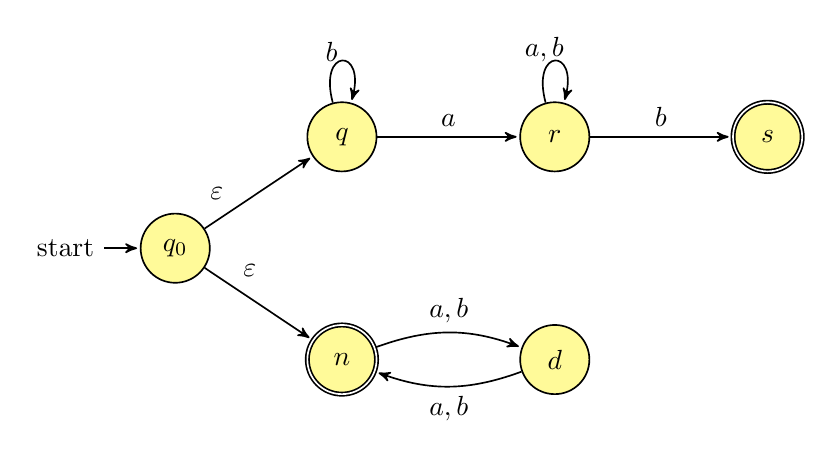
\begin{tikzpicture}[->,>=stealth',shorten >=1pt, auto, node distance=2cm, semithick]
    \tikzstyle{every state}=[text=black, fill=yellow!40]
    
    \node[initial,state] (q0)          {$q_0$};
    \node[state]         (q) [above right of=q0, xshift=20pt] {$q$};
    \node[state]         (r) [right of=q, xshift=20pt] {$r$};
    \node[state, accepting]         (s) [right of=r, xshift=20pt] {$s$};
    \node[state, accepting]         (n) [below right of=q0, xshift=20pt] {$n$};
    \node[state]         (d) [right of=n, xshift=20pt] {$d$};
    
    \path (q0) edge  [bend left=0, near start] node {$\varepsilon$} (q)
            edge [bend right=0, near start] node {$\varepsilon$} (n)
        (q) edge [bend left=0] node {$a$} (r)
            edge [loop above, near start] node {$b$} (q)
        (r) edge [bend left=0] node {$b$} (s)
            edge [loop above, near start] node {$a,b$} (r)
        (n) edge [bend left=20] node {$a,b$} (d)
        (d) edge [bend left=20] node {$a,b$} (n)
    ;
    \end{tikzpicture}
is:


\newpage

Could we do the same construction with DFA?

\vspace{50pt}

Happily, though, an analogous claim is true!

Suppose $A_1, A_2$ are languages over an alphabet $\Sigma$.
{\bf Claim:} if there is a DFA $M_1$ such that $L(M_1) = A_1$ and 
DFA $M_2$ such that $L(M_2) = A_2$, then there is another DFA, let's call it $M$, such that 
$L(M) = A_1 \cup A_2$. {\it Theorem 1.25 in Sipser, page 45}
    
    {\bf Proof idea}:
    
    
    {\bf Formal construction}: 
    
    \vfill

    
    {\bf Example}:  When $A_1 = \{w \mid w~\text{has an $a$ and ends in $b$} \}$ and 
    $A_2 = \{ w \mid w~\text{is of even length} \}$.
    
    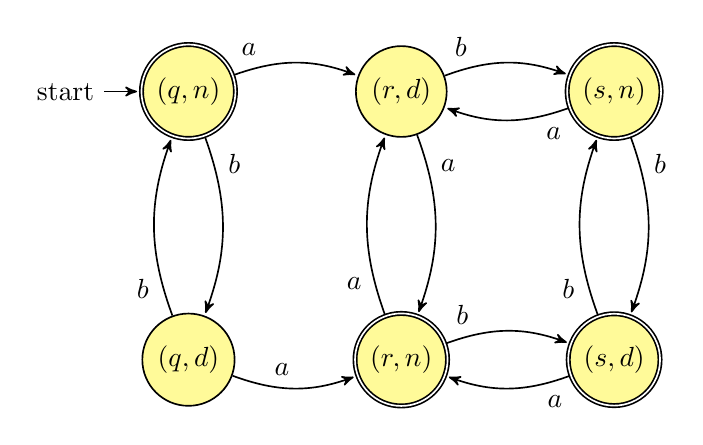
\begin{tikzpicture}[->,>=stealth',shorten >=1pt, auto, node distance=2cm, semithick]
        \tikzstyle{every state}=[text=black, fill=yellow!40]
        
        \node[initial,state,accepting] (qn)          {$(q,n)$};
        \node[state]         (qd) [below of=qn, yshift=-40pt] {$(q,d)$};
        \node[state]         (rd) [right of=qn, xshift=20pt] {$(r,d)$};
        \node[state,accepting]         (rn) [right of=qd, xshift=20pt] {$(r,n)$};
        \node[state,accepting]         (sn) [right of=rd, xshift=20pt] {$(s,n)$};
        \node[state,accepting]         (sd) [right of=rn, xshift=20pt] {$(s,d)$};
        
        \path (qn) edge  [bend left=20, near start] node {$b$} (qd)
                edge [bend left=20, near start] node {$a$} (rd)
            (qd) edge [bend left=20, near start] node {$b$} (qn)
                edge [bend right=20, near start] node {$a$} (rn)
            (rn) edge [bend left=20, near start] node {$a$} (rd)
                edge [bend left=20, near start] node {$b$} (sd)
            (rd) edge [bend left=20, near start] node {$a$} (rn)
                edge [bend left=20, near start] node {$b$} (sn)
            (sn) edge [bend left=20, near start] node {$a$} (rd)
                edge [bend left=20, near start] node {$b$} (sd)
            (sd) edge [bend left=20, near start] node {$a$} (rn)
                edge [bend left=20, near start] node {$b$} (sn)
        ;
        \end{tikzpicture}
    
    \newpage
    
    Suppose $A_1, A_2$ are languages over an alphabet $\Sigma$.
    {\bf Claim:} if there is a DFA $M_1$ such that $L(M_1) = A_1$ and 
    DFA $M_2$ such that $L(M_2) = A_2$, then there is another DFA, let's call it $M$, such that 
    $L(M) = A_1 \cap A_2$.  {\it Sipser Theorem 1.25, page 45}
    
    {\bf Proof idea}:
    
    
    {\bf Formal construction}: 
    
    \vspace{70pt}


    
 

\end{document}